\documentclass[11pt]{article}
\pagestyle{plain}
\usepackage{preamble}

\begin{document}
\section{Algorithme du \emph{solver}}
Le but de ce devoir était d'implémenter une factorisation QR, et de résoudre un système linéaire donné sous forme matricielle utilisant celle-ci.
L'implémentation est divisée en deux parties:
\begin{itemize}
	\item La fonction \texttt{QR} qui calcule, pour une matrice $A \in \mathbb{R}^{m \times n}$, la matrice triangulaire supérieure $R \in \mathbb{R}^{n \times n}$, ainsi qu'une matrice $V$ reprenant les différents réflecteurs de Householder.
	\item La fonction \texttt{QRsolve}, qui résout le système $Ax = b$ en utilisant la fonction \texttt{QR} pour factoriser $A$, et qui utilise ensuite une substitution arrière pour trouver $x$, sans devoir calculer explicitement $Q$. 
\end{itemize}

\section{Complexité}
\label{sec:complexity}
\fbox{\texttt{QR}} La complexité de la fonction \texttt{QR} % TODO voir livre

\fbox{\texttt{QRsolve}} Dans la fonction \texttt{QRsolve}, on fait appel à \texttt{QR},
cependant dans cette section on détaille uniquement le coût algorithmique propre à la fonction.
Celui-ci est dominé par la substitution arrière,
dont la complexité est
\[
b(n) \sim \sum_{j=1}^{n} \big(2(n - j) + 1 \big) \sim 2 \sum_{k=0}^{n-1} k + n \sim n (n - 1) + n \sim n^2\,.
\]

\fbox{Totale} Comme la complexité $t(m, n)$ qui nous intéresse ici est asymptotique,
et que \texttt{QRsolve} et \texttt{QR} se font séquentiellement,
on peut laisser tomber les termes d'ordre inférieur dus à la substitution arrière.
On obtient donc une complexité totale
\[
t(m, n) \sim 2 mn^2 - \frac{2}{3}n^3 + n^2 \sim 2mn^2 - \frac{2}{3}n^3 \overset{m = n}{\implies} t(n) \sim \frac{4}{3} n^3\,.\ 
\]
Si on construit le graphe donnant le temps d'exécution en fonction de la taille de l'entrée en échelle logarithmique,
on s'attend donc à avoir une pente de $3$, car $\log n^d = d \log n$.
\section{Résultats}
Afin de vérifier la bonne implémentation de l'algorithme,
celui-ci a été testé en comparant les résultats avec ceux de \texttt{np.linalg.solve}.
On remarque que sur les graphes log-log,
la pente pour les deux solvers est très proche de $3$,
ce qui correspond à la prédiction faite à la section~\ref{sec:complexity}.
Notons cependant que \texttt{np.linalg.solve} est plus rapide d'un facteur $\approx \num{10000}$,
car il s'agit d'une implémentation basée sur l'algorithme de décomposition LU plus efficace
et car cet algorithme est implémenté en Fortran (LAPACK), un langage beaucoup plus bas niveau que Python.

À cause de cette différence d'ordre de grandeur, le solver de \texttt{NumPy} est plus sensible aux autres tâches effectuées par le processeur.
On remarque en effet que les points sont moins regroupés (surtout pour les petites valeurs) que pour le graphe de \texttt{QRsolve}.

\begin{figure}[H]
	\centering
	\begin{subfigure}{0.33\textwidth}
		\centering
		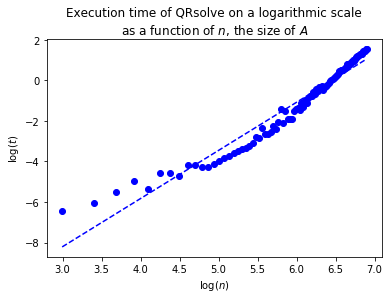
\includegraphics[width=\linewidth]{hw1_loglog_qr.png}
		\caption{\texttt{QRsolve}, échelle logarithmique.}
		\label{fig:llqr}
	\end{subfigure}%
	\begin{subfigure}{0.33\textwidth}
		\centering
		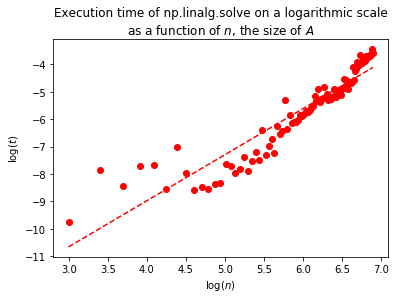
\includegraphics[width=\linewidth]{hw1_loglog_np.png}
		\caption{\texttt{NumPy}, échelle logarithmique.}
		\label{fig:llnp}
	\end{subfigure}
	\begin{subfigure}{0.33\textwidth}
		\centering
		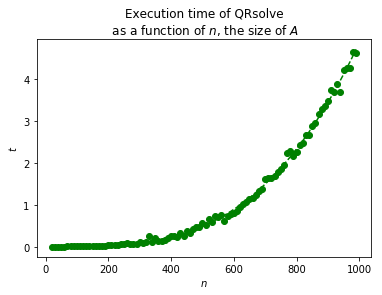
\includegraphics[width=\linewidth]{hw1_cubic.png}
		\caption{\texttt{QRsolve}, échelle linéaire.}
		\label{fig:cubic}
	\end{subfigure}
	\caption{Graphes du temps d'exécution en fonction de la taille d'entrée sur différentes échelles.}
	\label{fig:manmade}
\end{figure}
\end{document}
